\documentclass[12pt]{article}
\usepackage[margin=0.8in]{geometry}
\usepackage[utf8]{inputenc}
\usepackage{tikz}
\usepackage{graphicx}
\usepackage{amsmath}
\usepackage[version=4]{mhchem}
\usepackage{siunitx}
\usepackage{longtable,tabularx}
\usepackage{cleveref}
\setlength\LTleft{0pt} 
\usepackage{subcaption}
\usepackage{relsize}
\usepackage{float}
\usepackage{booktabs}
\usepackage{bm}
\usepackage{comment}
\graphicspath{ {./Figures/} }
\usepackage{amssymb}
\usepackage{listings}
\usepackage{color} %red, green, blue, yellow, cyan, magenta, black, white
\definecolor{mygreen}{RGB}{28,172,0} % color values Red, Green, Blue
\definecolor{mylilas}{RGB}{170,55,241}

\date{} 
\title{Project 1 \large \\
        Statistical Patter Recognition}

\author{Girguis Sedky} 
\begin{document}
\maketitle


\section{ML/Bayes rule estimation}
In this method, the image pixel values were assumed to have a gaussian distribution. In addition, the prior probability of all the classes were assumed to be equal during training and testing. Under this assumption, the Bayesian classification rule reduces to assigning a state to the class that maximizes 

\begin{equation}
P(\bm{x}|\omega_i) = \frac{1}{((2\pi)^d |\Sigma|)^{1/2}}\exp\left(-\frac{1}{2}(\bm{x}-\bm{\mu})^{\text{T}}\Sigma^{-1}(\bm{x}-\bm{\mu})\right),
\end{equation}  
where $d=784$ is the length of the state vectors. This is equivalent to maximizing
\begin{equation}
\log\left(P(\bm{x}|\omega_i)\right) = -\frac{1}{2}\log(|\Sigma|)- \frac{1}{2}(\bm{x}-\bm{\mu})^{\text{T}}\Sigma^{-1}(\bm{x}-\bm{\mu}).
\end{equation} 
The sample mean and covariances for each class are
\begin{equation}
\bm{\hat{\mu}}_i = \frac{1}{n}\sum_{j=1}^{n}\bm{x}_j,
\end{equation}
\begin{equation}
\hat{\Sigma}_i = \frac{1}{n}\sum_{j=1}^{n}(\bm{x}_j-\bm{\hat{\mu}}_i)(\bm{x}_j-\bm{\hat{\mu}}_i)^{\text{T}}.
\end{equation}
A training script was used on the training set comprised of 60,000 images to determine $\bm{\hat{\mu}}_i$ and $\hat{\Sigma}_i$ of every class and a testing script in turn used these values and the Bayesian classification algorithm to classify the test images.

Since the covariance matrices are large and some are singular, special computational techniques were used to ensure good results. A pseudo inverse operation was used to inverse $|\Sigma_i|$ and small multiple of the identity was added to $|\Sigma_i|$ before obtaining its determinant. \textbf{The classification error on the testing set came to about $35 \%$}


\section{Nearest Neighborhood classifier}
In this method, the image pixel values are arranged in a single column vector that lives in $\mathbb{R}^{784}$. In this space, each training image constitutes a prototype. The euclidiean distance between each testing image and all the training images is found, and the testing image is assigned to the class of the training image that is closest to it. \textbf{The classification error on the testing set came to about $15 \%$}

\section{PCA/LDA}
\subsection{PCA}
Principal component analysis was used to reduce the dimensionality of the problem. The low-order state vectors were then fed into the Bayesian and Nearest Neighborhood classifier. Figure~\ref{fig:PCA} demonstrates the percentage error in classification based on the number of dimensions kept. \textbf{The minimum classification error came to about $ 20.5\%$ for 50 kept components in the case of the Bayesian classifier and $14.7 \%$ for 150 components kept in the case of the Nearest Neighborhood classier.}
 \begin{figure}[h]
 \centering
 \begin{subfigure}[H]{0.49\textwidth}
\centering
  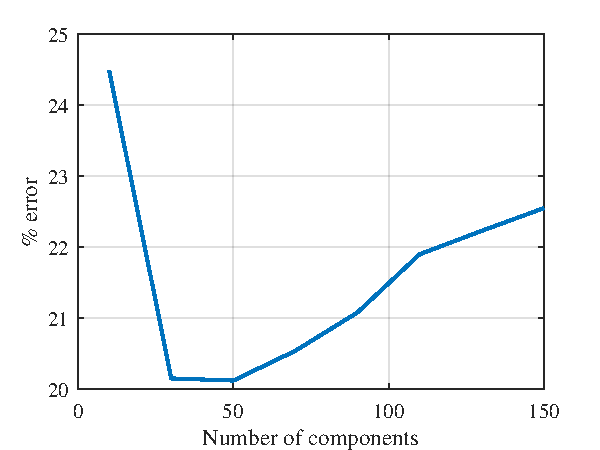
\includegraphics[width=\linewidth]{ML_PCA.pdf}
  \caption{Bayesian classifier}
  
\end{subfigure}
 \begin{subfigure}[H]{0.49\textwidth}
\centering
  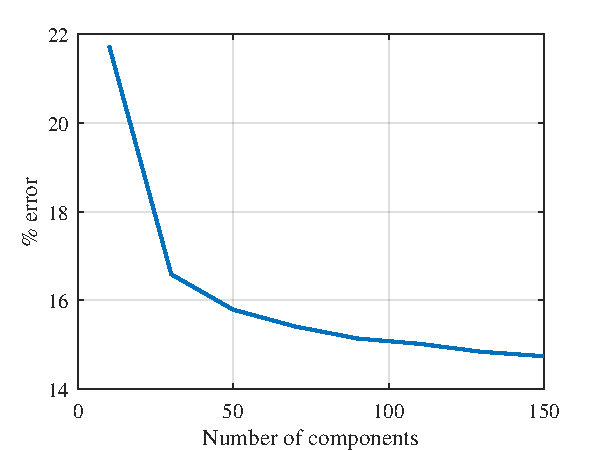
\includegraphics[width=\linewidth]{NN_PCA.pdf}
  \caption{Nearest neighborhood classifier}
  
  \end{subfigure}
  \caption{Principal component analysis}
  \label{fig:PCA}
\end{figure}
\subsection{LDA}
Linear discriminant analysis was used to reduce the image state vectors from $\mathbb{R}^{784}$ to $\mathbb{R}^{M-1}$ where $M$ is the number of classes. The built-in MATLAB function was used for this purpose. Again, the low-order state vectors were then fed into the Bayesian and Nearest Neighborhood classifier. \textbf{The minimum classification error came to about $ 25.4\%$ in the case of the Bayesian classifier and $28 \%$ in the case of the Nearest Neighborhood classier.}
\newpage
\section{Summary}
Table~\ref{table:1} shows the classification error of the different methods utilized in this study. The most accurate method of classification was to use principal component analysis to reduce the dimensionality of the state vectors to 50 and then to apply NN to the transformed data.
\begin{table}[H]
\centering
\caption{Summary of classification results}
\label{table:1}
\begin{tabular}{cc}
\hline
Method     & Percentage Error \\ \hline
Bayes      & 35\%             \\
NN         & 15\%             \\
PCA, Bayes (50) & 20.5\%           \\
PCA, NN  (150)  & 14.7\%           \\
LDA, Bayes & 25.4\%           \\
LDA, NN    & 28\%             \\ \hline
\end{tabular}
\end{table}


\lstset{language=Matlab,%
    %basicstyle=\color{red},
    breaklines=true,%
    morekeywords={matlab2tikz},
    keywordstyle=\color{blue},%
    morekeywords=[2]{1}, keywordstyle=[2]{\color{black}},
    identifierstyle=\color{black},%
    stringstyle=\color{mylilas},
    commentstyle=\color{mygreen},%
    showstringspaces=false,%without this there will be a symbol in the places where there is a space
    numbers=left,%
    numberstyle={\tiny \color{black}},% size of the numbers
    numbersep=9pt, % this defines how far the numbers are from the text
    emph=[1]{for,end,break},emphstyle=[1]\color{red}, %some words to emphasise
    %emph=[2]{word1,word2}, emphstyle=[2]{style},    
}

\newpage
\section*{Appendix}
\subsection*{ML/Bayes rule estimation}
\subsubsection*{Training script}
\lstinputlisting{TrainingScript_ML.m}

\subsubsection*{Testing script}
\lstinputlisting{TestingScript_ML.m}

\subsection*{NN}
\lstinputlisting{NN.m}

\subsection*{PCA}
\subsection{ML/Bayes rule estimation with PCA}
\lstinputlisting{ML_PCA.m}

\subsection{NN with PCA}
\lstinputlisting{NN_PCA.m}

\subsection*{LDA}
\lstinputlisting{LDA_Script.m}


\end{document}